% Created 2018-04-09 lun 18:27
% Intended LaTeX compiler: pdflatex
\documentclass[xcolor={usenames,svgnames,dvipsnames}]{beamer}
\usepackage[utf8]{inputenc}
\usepackage[T1]{fontenc}
\usepackage{graphicx}
\usepackage{grffile}
\usepackage{longtable}
\usepackage{wrapfig}
\usepackage{rotating}
\usepackage[normalem]{ulem}
\usepackage{amsmath}
\usepackage{textcomp}
\usepackage{amssymb}
\usepackage{capt-of}
\usepackage{hyperref}
\usepackage{color}
\usepackage{listings}
\usepackage{mathpazo}
\usepackage{gensymb}
\usepackage{amsmath}
\usepackage{chemarr}%flechas para reacciones químicas (SFER.tex)
\bibliographystyle{plain}
\AtBeginSubsection[]{\begin{frame}[plain]\tableofcontents[currentsubsection,sectionstyle=show/shaded,subsectionstyle=show/shaded/hide]\end{frame}}
\AtBeginSection[]{\begin{frame}[plain]\tableofcontents[currentsection,hideallsubsections]\end{frame}}
\usepackage[emulate=units]{siunitx}
\sisetup{fraction=nice, decimalsymbol=comma, retain-unity-mantissa = false}
\newunit{\wattpeak}{Wp}
\newunit{\watthour}{Wh}
\newunit{\amperehour}{Ah}
\hypersetup{colorlinks=true, linkcolor=Blue, urlcolor=Blue}
\renewcommand{\thefootnote}{\fnsymbol{footnote}}
\beamertemplatenavigationsymbolsempty
\setbeamertemplate{footline}[frame number]
\setbeamercolor{alerted text}{fg=blue!50!black} \setbeamerfont{alerted text}{series=\bfseries}
\usetheme[hideothersubsections]{Goettingen}
\usecolortheme{rose}
\usefonttheme{serif}
\author{Oscar Perpiñán Lamigueiro \\ \url{http://oscarperpinan.github.io}}
\date{}
\title{SFCR: Diseño}
\hypersetup{
 pdfauthor={Oscar Perpiñán Lamigueiro \\ \url{http://oscarperpinan.github.io}},
 pdftitle={SFCR: Diseño},
 pdfkeywords={},
 pdfsubject={},
 pdfcreator={Emacs 25.2.2 (Org mode 9.1.9)}, 
 pdflang={Spanish}}
\begin{document}

\maketitle

\section{Generador Fotovoltaico}
\label{sec:org9680044}

\begin{frame}[label={sec:orge962670}]{Inclinación y Orientacion}
$$\beta_{opt}=3.7+0.69 \cdot \left|\phi\right|$$

\begin{center}
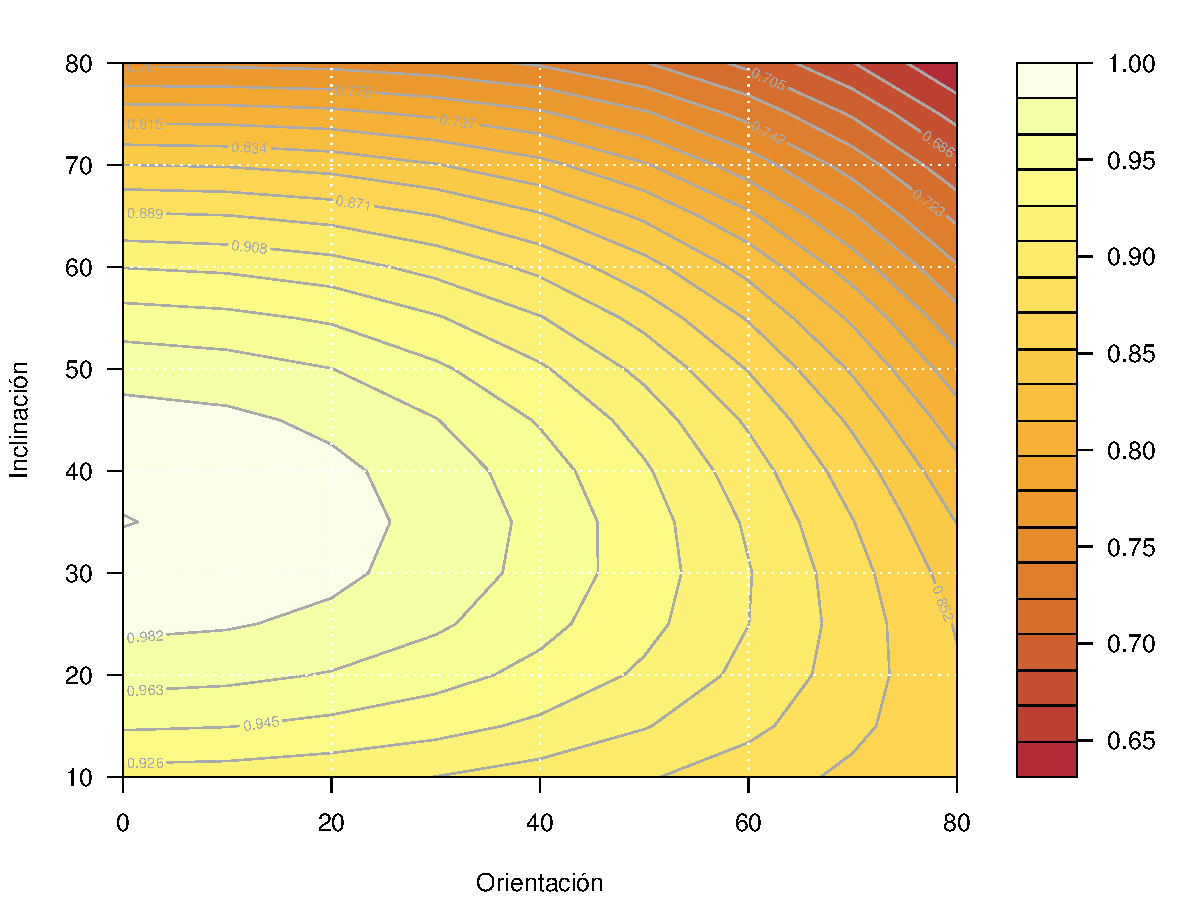
\includegraphics[width=.9\linewidth]{../figs/PorcentajeProduccionEdificios.pdf}
\end{center}
\end{frame}

\begin{frame}[label={sec:org5ceec8b}]{Modulos en serie}
\begin{itemize}
\item El inversor está diseñado para soportar una \alert{tensión máxima en la
entrada}. Superarla puede conllevar la avería del equipo.
\end{itemize}

$$N_{s,max}:\, V_{ocG}(G=\SI{200}{\watt\per\meter\squared},\,
T_{a}=\SI{-10}{\celsius})<V_{max,inv}$$

\begin{itemize}
\item Por otra parte, el algoritmo de \alert{búsqueda del MPP} se realiza en un
rango de tensiones limitado. Para evitar pérdidas por trabajar en un
punto alejado del MPP, la tensión del generador debe estar dentro de
este rango.
\end{itemize}

$$N_{s,mpp}:\, V_{mppG}(G_{stc},\,
T_{a}=\SI{25}{\celsius})\in\left[V_{mppMIN},\,
  V_{mppMAX}\right]_{INV}$$
\end{frame}

\begin{frame}[label={sec:orga73fe74}]{Ramas en paralelo}
\begin{itemize}
\item El fabricante del inversor elige los componentes para soportar una \alert{corriente máxima admisible}.

\item En general, el inversor es capaz de autoprotegerse ante valores superiores a este umbral desplazando el punto de funcionamiento del generador fuera del MPP.

\item No obstante, el diseñador del sistema debe elegir el número de ramas en paralelo de forma que no se supere este umbral.
\end{itemize}

$$N_{p,max}:\, I_{scG}(\SI{1000}{\watt\per\meter\squared})<I_{max,INV}$$
\end{frame}

\begin{frame}[label={sec:org4b285aa}]{Configuración del generador}
De los cálculos anteriores se obtiene un conjunto de configuraciones del generador que permiten un buen acoplamiento entre inversor y generador. 

Para elegir una configuración deben tenerse en cuenta diferentes aspectos:

\begin{itemize}
\item Configuración eléctrica y ubicación física de los módulos en la
estructura.

\item La curva de eficiencia del inversor depende de la tensión de entrada.

\item Inversión y rendimiento económicos.

\item Espacio disponible.

\item Relación de potencias de generador e inversor.
\end{itemize}
\end{frame}

\begin{frame}[label={sec:org0e44366}]{Configuración eléctrica y estructura}
\begin{itemize}
\item Es recomendable elegir \alert{series} compuestas por un número de módulos
que puedan ser ubicados en una \alert{única hilera de la estructura}.

\begin{itemize}
\item \alert{Se facilita el trazado del cableado}: la propia estructura puede
servir como fijación auxiliar, se evitan cruzamientos indeseados.

\item \alert{Se minimiza la influencia de las sombras}: es muy frecuente la
aparición de sombras entre partes del generador o entre
seguidores, sombras de forma rectangular y que comienzan afectando
a las partes bajas de la estructura. Al cablear por hileras, las
sombras de las hileras bajas no afectan a las hileras
inmediatamente superiores.
\end{itemize}
\end{itemize}
\end{frame}

\begin{frame}[label={sec:orgdc53ea2}]{Potencia del generador}
\begin{itemize}
\item La potencia del generador fotovoltaico está relacionada directamente
con la \alert{inversión económica} a realizar.

\item Por otra parte, la relación entre \alert{energía generada} y potencia
nominal es aproximadamente lineal, y por tanto, los \alert{ingresos
económicos} dependen casi linealmente de la potencia del generador.

\item Por tanto, para decidir la potencia del generador
(\(P_{g}^{*}=N_{s}\cdot N_{p}\cdot P_{m}^{*}\)) debe tenerse en cuenta
el capital o financiación disponible, y el rendimiento económico
deseado.
\end{itemize}
\end{frame}

\begin{frame}[label={sec:org118369f}]{Potencia del generador}
\begin{itemize}
\item La potencia del generador es proporcional al área del generador y al \alert{terreno ocupado} (que también influye, aunque en menor grado, en el    cálculo económico). Por tanto, debe tenerse en cuenta el espacio disponible (o el coste que se pretende asumir por el uso de terreno).

\item Según el \alert{tipo de sistema} (estático, seguimiento) se debe elegir una relación de potencias de generador e inversor.
\end{itemize}
\end{frame}

\section{Inversor}
\label{sec:orga899828}

\begin{frame}[label={sec:orgeebe35d}]{Curva de eficiencia}
\begin{itemize}
\item Eficiencia del inversor, \(\eta_{inv} = P_{ac} / P_{dc}\)

\item Esta relación puede describirse con una función basada en tres coeficientes y la normalización de la potencia de salida, \(p_{o}=P_{ac}/P_{inv}\): $$\eta_{inv}=\frac{p_{o}}{p_{o}+k_{0}^{o}+k_{1}^{o}p_{o}+k_{2}^{o}p_{o}^{2}}$$
\end{itemize}
\end{frame}


\begin{frame}[label={sec:org22dff68}]{Curva de eficiencia}
\(k_{0}^{o}=0.01\)

\(k_{1}^{o}=0.025\)

\(k_{2}^{o}=0.05\)

\begin{center}
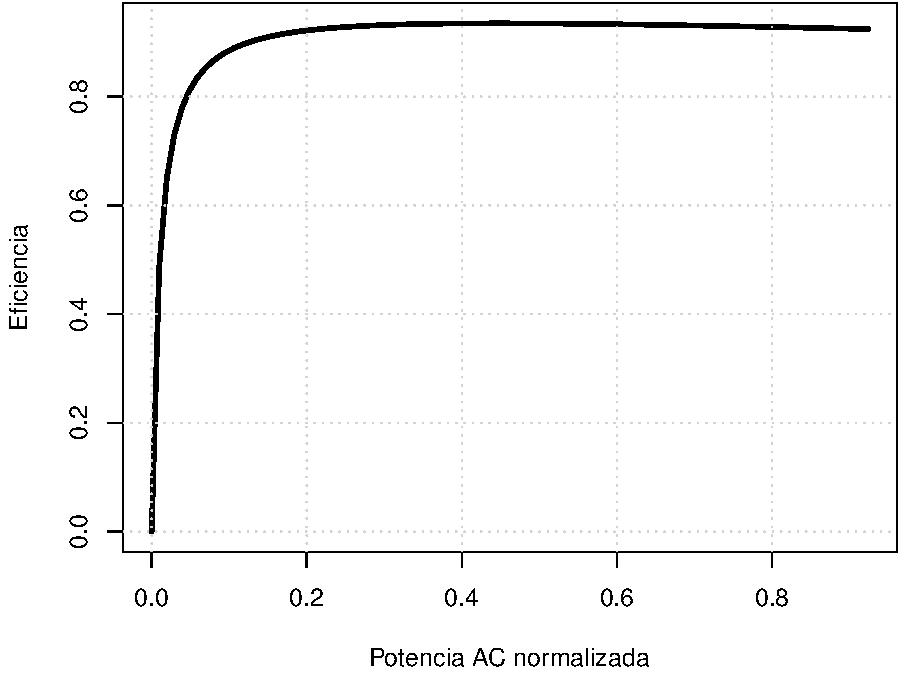
\includegraphics[width=.9\linewidth]{../figs/CurvaInversor.pdf}
\end{center}
\end{frame}

\begin{frame}[label={sec:org2b0f439}]{Relación de potencias}
\begin{itemize}
\item Dado que la potencia entregada por el generador varía con las condiciones meteorológicas, el inversor trabajará en diferentes zonas de su curva de eficiencia.

\item Por tanto, una de las preguntas a responder es \alert{que relación debe existir entre la potencia del generador FV y el inversor}.

\[F_{DI} = P_{g}^{*}/P_{inv}\]

\item Si esta relación es alta, el inversor trabajará con frecuencia en la región de alta eficiencia, pero a cambio es posible que deba limitar la potencia del generador para evitar superar su umbral de corriente admisible.
\end{itemize}
\end{frame}

\begin{frame}[label={sec:orgba0b618}]{Relación de potencias}
\begin{itemize}
\item En \alert{sistemas de integración arquitectónica}, donde la orientación e inclinación no son óptimas, esta probabilidad puede ser baja. Así, puede considerarse necesario sobredimensionar el generador FV respecto al inversor (\(P_{g}^{*}/P_{inv}\in\left[1;1.4\right]\)).

\begin{itemize}
\item CTE-HE5-3.2.3.2: \guillemotleft{}la potencia del inversor será como mínimo el 80\% de la potencia pico real del generador fotovoltaico\guillemotright{}
\end{itemize}

\item En \alert{sistemas de seguimiento} esta probabilidad suele ser alta. Se recomiendan inversores de potencia similar a la del generador  (\(P_{g}^{*}/P_{inv}\in\left[1;1.2\right]\))
\end{itemize}
\end{frame}

\begin{frame}[label={sec:org34aa765}]{Relación de potencias}
No obstante, es posible demostrar que el valor de esta relación no es tan crítico como \alert{elegir un inversor con buena curva de eficiencia}.
\end{frame}

\section{Cableado}
\label{sec:org52a8943}

\begin{frame}[label={sec:org4b2c875}]{Características básicas}
\begin{itemize}
\item Diseño del cableado

\begin{itemize}
\item Criterio de caída de tensión

\item En sistemas de gran tamaño reducir bucles

\item Diseño de estructura e integración: habilitar un camino para
cableado
\end{itemize}

\item Tipo de cables

\begin{itemize}
\item Doble aislamiento

\item Poliolefínas
\end{itemize}
\end{itemize}
\begin{center}
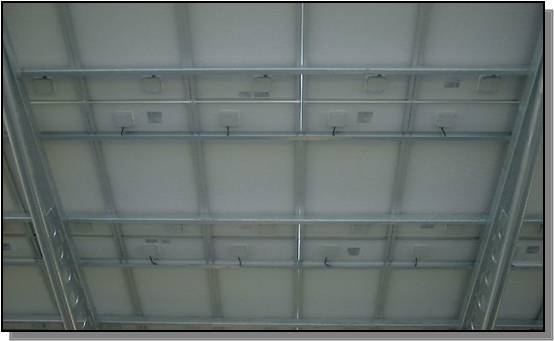
\includegraphics[height=0.5\textheight]{../figs/PhotocampaCableado.jpg}
\end{center}
\end{frame}

\begin{frame}[label={sec:orgea75e27}]{Cálculo}
\begin{itemize}
\item Habitualmente se descarta el criterio termico y se emplea el criterio de caida de tensión (RBT ITC-BT-07):
\end{itemize}

\[
  \begin{aligned}
    S_{dc} & = & \frac{2 \cdot L_{dc}\cdot I_{dc}}{\gamma_\theta \cdot \Delta V_{dc}}\\
    S_{1ac} & = & \frac{2\cdot L_{1ac}\cdot I_{1ac}}{\gamma_\theta \cdot \Delta V_{1ac}}\\
    S_{3ac} & = & \frac{\sqrt{3} \cdot L_{3ac}\cdot I_{3ac}}{\gamma_\theta \cdot \Delta V_{3ac}}
  \end{aligned}
\]

\begin{itemize}
\item La conductividad del cable, \(\gamma_\theta\), depende del material y de la
temperatura de operación. Por ejemplo, el cobre:
\begin{itemize}
\item \(\gamma_{20} =\SI{56}{\meter\per\ohm\per\milli\meter\squared}\)
\item \(\gamma_{70} = \SI{48}{\meter\per\ohm\per\milli\meter\squared}\).
\end{itemize}
\end{itemize}
\end{frame}

\begin{frame}[label={sec:org1fc835d}]{Cálculo}
\begin{itemize}
\item En general, se exige una caída máxima de tensión
\(\SI{1.5}{\percent}\) de la tensión nominal.

\item Para aplicar correctamente este porcentaje es importante caer en la
cuenta de que \alert{cada zona (DC y AC) tiene su propia tensión nominal}.
\end{itemize}
\end{frame}

\begin{frame}[label={sec:orgd6bea81}]{Cálculo}
\begin{block}{Ejemplo}
\begin{itemize}
\item En una instalación que conduce \(\SI{75}{\ampere}\) a la salida de un
inversor trifásico, situado este a \(\SI{100}{\meter}\) de la conexión
a red, se deberá utilizar un cable de sección (teniendo en cuenta
que \(\gamma_{70} = \SI{48}{\meter\per\ohm\per\milli\meter\squared}\)).
\end{itemize}


\[
  S=\frac{\sqrt{3} \cdot 100 \cdot 75}{48 \cdot \SI{1.5}{\percent}\cdot400}=\SI{45.46}{\milli\meter\squared}
\]

\begin{itemize}
\item Dado que la sección de los cables está normalizada, se deberá optar
por la sección inmediatamente superior, y por tanto la conexión del
inversor a la red se realizará con tres cables de sección
\(S=\SI{50}{\milli\meter\squared}\).
\end{itemize}
\end{block}
\end{frame}

\begin{frame}[label={sec:orgb6a6550}]{Intensidad máxima admisible}
\begin{itemize}
\item Con este resultado, es necesario comprobar que la intensidad de diseño es inferior a la intensidad máxima admisible del cable para sus condiciones de servicio, según las tablas de la ITC-BT-07.

\item No obstante, las secciones que resultan del criterio de caída de tensión aplicado a los sistemas fotovoltaicos habitualmente son sobradamente capaces de conducir la corriente del sistema.
\end{itemize}
\end{frame}

\begin{frame}[label={sec:org72ec9f0}]{Continua vs. Alterna}
\begin{block}{}
Suponiendo que en una planta con varios inversores trifásicos existe la
posibilidad de ubicar los inversores debajo del generador FV
(\emph{distribución en alterna}) o en un centro específico junto al punto de
conexión a red (\emph{distribución en continua}), \alert{¿cuál es la tensión de
trabajo en continua que permite optar por una distribución en continua?}
\end{block}
\end{frame}
\end{document}